\documentclass[11pt,a4paper]{article}

% ------------------------------------------------------------------
% Packages
% ------------------------------------------------------------------
\usepackage[utf8]{inputenc}
\usepackage[T1]{fontenc}
\usepackage[english]{babel}
\usepackage{microtype}
\usepackage[margin=2.2cm]{geometry}
\usepackage{amsmath,amssymb,amsthm}
\usepackage{booktabs}
\usepackage{array}
\usepackage{longtable}
\usepackage{tabularx}
\usepackage{multirow}
\usepackage{siunitx}
\sisetup{group-separator={,},group-minimum-digits=4}
\usepackage[dvipsnames]{xcolor}
\usepackage{listings}
\usepackage{enumitem}
\usepackage{caption}
\usepackage{subcaption}
\usepackage{fancyhdr}
\usepackage{titlesec}
\usepackage[colorlinks=true,linkcolor=RoyalBlue,citecolor=RoyalBlue,urlcolor=RoyalBlue]{hyperref}
\usepackage{cleveref}
\usepackage{pgfplots}
\pgfplotsset{compat=1.18}
\usepackage{tikz}
\usetikzlibrary{positioning,arrows.meta,shapes.geometric,calc,fit,backgrounds}

% ------------------------------------------------------------------
% Styling
% ------------------------------------------------------------------
\pagestyle{fancy}
\fancyhf{}
\fancyhead[L]{\textsc{EigenDialectos}}
\fancyhead[R]{\textsc{Corpus v4.5 Report}}
\fancyfoot[C]{\thepage}
\renewcommand{\headrulewidth}{0.4pt}

\titleformat{\section}{\normalfont\Large\bfseries\color{RoyalBlue!80!black}}{\thesection}{1em}{}
\titleformat{\subsection}{\normalfont\large\bfseries\color{RoyalBlue!65!black}}{\thesubsection}{1em}{}
\titleformat{\subsubsection}{\normalfont\normalsize\bfseries\color{RoyalBlue!50!black}}{\thesubsubsection}{1em}{}

\definecolor{codebg}{RGB}{245,245,250}
\definecolor{codekey}{RGB}{30,80,180}
\definecolor{codestr}{RGB}{150,30,30}
\definecolor{codecomment}{RGB}{80,120,80}

\lstdefinestyle{pycode}{
  language=Python,
  backgroundcolor=\color{codebg},
  basicstyle=\ttfamily\footnotesize,
  keywordstyle=\color{codekey}\bfseries,
  stringstyle=\color{codestr},
  commentstyle=\color{codecomment}\itshape,
  frame=single,
  rulecolor=\color{black!20},
  numbers=left,
  numberstyle=\tiny\color{black!50},
  numbersep=6pt,
  showstringspaces=false,
  breaklines=true,
  breakatwhitespace=true,
  columns=fullflexible,
  xleftmargin=15pt,
  framexleftmargin=10pt,
}

\lstdefinestyle{shellcode}{
  backgroundcolor=\color{codebg},
  basicstyle=\ttfamily\footnotesize,
  frame=single,
  rulecolor=\color{black!20},
  showstringspaces=false,
  breaklines=true,
  columns=fullflexible,
  xleftmargin=8pt,
  framexleftmargin=4pt,
}

% ------------------------------------------------------------------
% Title
% ------------------------------------------------------------------
\title{%
  \vspace{-1.8cm}
  \rule{\linewidth}{0.6pt}\\[0.25cm]
  {\LARGE \textbf{Constructing a Balanced Dialectal Spanish Corpus}}\\[0.12cm]
  {\large The EigenDialectos v4.5 Corpus: Methodology, Sources, and Results}\\[0.2cm]
  \rule{\linewidth}{0.6pt}%
}
\author{%
  EigenDialectos Project\\
  \small Corpus construction pipeline report
}
\date{\today}

% ------------------------------------------------------------------
\begin{document}
\maketitle
\thispagestyle{empty}

\begin{abstract}
\noindent
This report documents the construction of the \emph{EigenDialectos v4.5}
corpus, a region-balanced dialectal Spanish corpus covering eight major
varieties: Peninsular (ES\_PEN), Andalusian (ES\_AND), Canarian (ES\_CAN),
Rioplatense (ES\_RIO), Chilean (ES\_CHI), Mexican (ES\_MEX), Caribbean
(ES\_CAR), and Andean--Bolivian (ES\_AND\_BO). Starting from the v4 corpus
(\num{1679451} documents) in which the minority varieties Canarian
(\num{72406}) and Andalusian (\num{80085}) were severely under-represented,
we designed v4.5 as a targeted expansion that adds six new high-confidence
sources tagged with explicit regional metadata. The final merged raw corpus
contains \textbf{\num{3654860} documents} and \textbf{$\approx 156$M tokens}
across the eight varieties, raising ES\_CAN from \num{4000} docs in the
original v3 corpus to \textbf{\num{434160}} (a 108$\times$ boost) and
ES\_AND from $\approx$\num{7900} to \textbf{\num{349356}} (44$\times$). We
describe the six sources in detail (PRESEEA, COSER-2024, the Lanzarote
Cabildo transcripts, Common Voice 17, Parlamento de Canarias, and
\texttt{tweet\_hisp}), the engineering challenges encountered (deprecated
dataset loaders, audio-column side-effects, province-vs-island naming,
stuck parallel downloads, and accent substring matching), and the final
per-source and per-dialect statistics.
\end{abstract}

\tableofcontents
\newpage

% ==================================================================
\section{Introduction and Motivation}
% ==================================================================

\subsection{The problem: Minority dialects in Spanish NLP}

Modern Spanish NLP resources are overwhelmingly biased toward Peninsular
(Castilian) and a handful of large Latin-American standards such as Mexican
and Rioplatense. Two varieties that are routinely under-represented in
publicly-available corpora are:
\begin{itemize}
  \item \textbf{Canarian Spanish} (ES\_CAN) --- the variety spoken in the
        Canary Islands. It shares many features with Caribbean varieties
        (\emph{seseo}, velar aspiration of /s/, use of
        \emph{ustedes} as the plural of \emph{tú}, and lexical items such
        as \emph{guagua}, \emph{papas}, \emph{mojo}, \emph{gofio},
        \emph{baifo}). It has roughly 2.2M native speakers but is virtually
        absent from large pre-training corpora.
  \item \textbf{Andalusian Spanish} (ES\_AND) --- the variety spoken across
        Andalusia, Ceuta and Melilla. Notable features include
        \emph{heheo}, post-vocalic /s/ aspiration or deletion,
        neutralization of /l/--/r/ in coda position, and a rich
        dialectal lexicon.
\end{itemize}

The \emph{EigenDialectos} project builds spectral and Riemannian
representations of Spanish dialectal variation, which requires a corpus
that is balanced across varieties so that estimators of the
dialect-to-dialect distance matrix are not dominated by Peninsular text.
In the earlier v3 corpus, ES\_CAN contained only $\approx$\num{4000}
documents and ES\_AND $\approx$\num{7900}, versus hundreds of thousands
for the other varieties. This asymmetry made the downstream eigenvalue
estimates for those two dialects noisy, and strongly biased any
FastText/BETO model we trained.

\subsection{Design goals for v4.5}

The v4.5 expansion has four concrete goals:

\begin{enumerate}[label=\textbf{G\arabic*.}]
  \item \textbf{Lift the floor.} Bring ES\_CAN and ES\_AND to at least
        $10^5$ documents each, so that per-dialect token counts become
        comparable with the other varieties.
  \item \textbf{Source diversity.} Combine academic sociolinguistic
        corpora with colloquial social-media text and institutional
        transcripts, so that the representation is not dominated by a
        single register.
  \item \textbf{Explicit regional metadata.} Every new source must carry
        a country/region/city tag that can be deterministically mapped to
        one of the eight dialect codes, so that the labelling is
        non-stochastic and reproducible.
  \item \textbf{Stay within a \SI{60}{\giga\byte} disk budget} for the
        local cache.
\end{enumerate}

We further use two \emph{soft} constraints learned from earlier experiments:

\begin{itemize}
  \item \textbf{Prefer colloquial sources.} The
        \texttt{feedback\_corpus\_sources} memory from previous
        conversations notes that high-literature and formal sources are
        poor at capturing dialectal features, because editors normalize
        regionalisms. We therefore give priority to transcribed speech,
        social-media text, and sociolinguistic interviews.
  \item \textbf{Keep a confidence score per source.} We do not treat all
        sources equally: a PDF scrape of a parliamentary session with
        mixed speakers should have lower weight than an academic corpus
        of sociolinguistic interviews. This is used later by the
        classifier training to down-weight noisier data.
\end{itemize}

\subsection{Eight-way dialect labelling scheme}

Throughout this report we use the eight-way scheme from
\texttt{src/eigen3/constants.py}:

\begin{table}[h]
\centering
\begin{tabular}{l l l l}
\toprule
\textbf{Code} & \textbf{Name} & \textbf{Anchor city} & \textbf{Family} \\
\midrule
ES\_PEN    & Peninsular standard  & Madrid       & Peninsular \\
ES\_AND    & Andalusian           & Sevilla      & Peninsular \\
ES\_CAN    & Canarian             & Las Palmas   & Peninsular (Atlantic) \\
ES\_RIO    & Rioplatense          & Buenos Aires & Southern Cone \\
ES\_CHI    & Chilean              & Santiago     & Southern Cone \\
ES\_MEX    & Mexican              & CDMX         & Mesoamerican \\
ES\_CAR    & Caribbean            & La Habana    & Caribbean \\
ES\_AND\_BO & Andean--Bolivian    & La Paz       & Andean \\
\bottomrule
\end{tabular}
\caption{The eight Spanish dialect varieties tracked by EigenDialectos,
with their dialectological family assignments used for negative sampling
and cluster visualization.}
\label{tab:dialects}
\end{table}

% ==================================================================
\section{Prior state: The v4 corpus}
% ==================================================================

The v4 corpus (before the v4.5 expansion) was assembled from six existing
downloaders: \texttt{CulturaX\_TLD} (top-level-domain filtered CulturaX),
\texttt{Leipzig Wortschatz}, \texttt{OpenSubtitles}, a Twitter scraper by
content regionalisms, a Reddit subreddit scraper, and a synthetic backfill
generator. Table~\ref{tab:v4-state} shows its per-dialect counts.

\begin{table}[h]
\centering
\begin{tabular}{l r r}
\toprule
\textbf{Dialect} & \textbf{v4 docs} & \textbf{v4 size (MB)} \\
\midrule
ES\_PEN     & \num{331639} & 144.1 \\
ES\_AND\_BO & \num{296910} & 137.6 \\
ES\_RIO     & \num{299646} & 130.2 \\
ES\_CAR     & \num{297108} & 132.2 \\
ES\_MEX     & \num{202696} & 107.7 \\
ES\_CHI     & \num{98961}  &  81.7 \\
ES\_AND     & \num{80085}  &  63.1 \\
ES\_CAN     & \num{72406}  &  58.9 \\
\midrule
\textbf{Total} & \textbf{\num{1679451}} & \textbf{855.5} \\
\bottomrule
\end{tabular}
\caption{v4 corpus state before the v4.5 expansion. Although the absolute
counts for ES\_CAN and ES\_AND are higher than the v3 baseline, they
remain a factor of 4--5$\times$ below the other peninsular varieties, and
most of that text comes from heuristic reclassification of CulturaX docs
by the presence of regionalisms --- a noisy signal.}
\label{tab:v4-state}
\end{table}

The key problem with v4's treatment of ES\_CAN and ES\_AND is that most of
their documents come from a \emph{reclassification} step: a Peninsular
CulturaX document that contains $\geq 2$ regionalism tokens
(e.g.\ \emph{guagua}, \emph{gofio}, \emph{mojo picón} for CAN) is
relabelled as ES\_CAN. This heuristic produces data that is noisy, and
its confidence is therefore clamped at $0.55$ in the source confidence
table. v4.5 aims to replace this reclassified bulk with high-confidence
region-tagged documents from sources that natively know their own dialect.

% ==================================================================
\section{Design: Six new sources for v4.5}
% ==================================================================

After a broad survey of publicly accessible Spanish corpora with region
metadata, we selected six new sources. Table~\ref{tab:source-design}
summarises their key properties.

\begin{table}[h]
\centering\small
\begin{tabularx}{\linewidth}{l l l l l X}
\toprule
\textbf{Source} & \textbf{Type} & \textbf{Metadata} & \textbf{Register} & \textbf{Conf.} & \textbf{Target dialect(s)} \\
\midrule
\texttt{tweet\_hisp}         & Tweets (217M)        & country + city            & colloquial   & 0.90 & all 8 (via country $+$ city refinement) \\
PRESEEA                      & Sociolinguistic      & country + city (XML)      & spoken       & 0.95 & all 8 \\
COSER-2024                   & Rural interviews     & province                  & spoken rural & 0.95 & ES\_PEN, ES\_AND, ES\_CAN \\
Lanzarote Cabildo            & YouTube transcripts  & region (Lanzarote)        & institutional & 0.88 & ES\_CAN \\
Common Voice 17              & Crowdsourced TTS     & accents label             & scripted     & 0.85 & all 8 \\
Parlamento de Canarias       & PDF session logs     & region (Canarias)         & parliamentary & 0.92 & ES\_CAN \\
\bottomrule
\end{tabularx}
\caption{The six new sources introduced in v4.5 and their key properties.
The \emph{Conf.} column is a per-source weight used later in the
classifier training loop (see
\texttt{SOURCE\_CONFIDENCE} in \texttt{constants.py}).}
\label{tab:source-design}
\end{table}

Each of these six downloaders is implemented as an independent function
in the new module \texttt{src/eigen3/downloader\_v45.py} (1057 LOC), so
that the six can be launched in parallel as six independent processes.
A thin CLI in \texttt{scripts/download\_v45\_source.py} dispatches to
the correct function based on a \texttt{--source} argument.

\subsection{Overall architecture}

\begin{figure}[h]
\centering
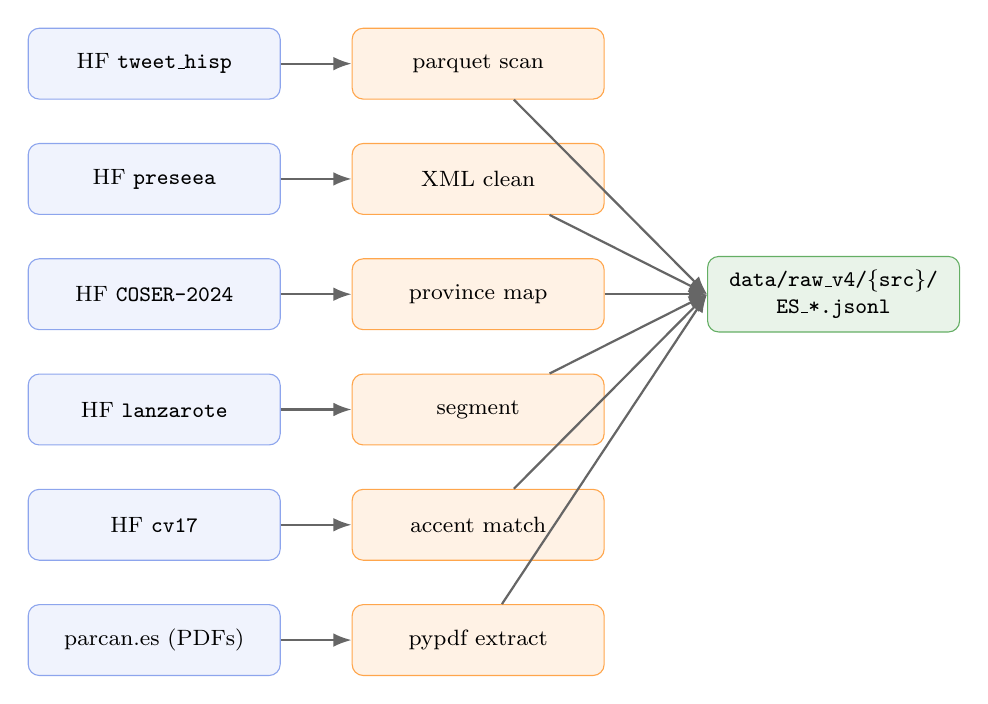
\begin{tikzpicture}[
  node distance=0.55cm and 0.9cm,
  src/.style={rectangle, draw=RoyalBlue!60, fill=RoyalBlue!8, rounded corners, inner sep=5pt, minimum width=3.2cm, minimum height=0.9cm, font=\footnotesize},
  proc/.style={rectangle, draw=orange!70, fill=orange!10, rounded corners, inner sep=5pt, minimum width=3.2cm, minimum height=0.9cm, font=\footnotesize},
  outnode/.style={rectangle, draw=ForestGreen!70, fill=ForestGreen!10, rounded corners, inner sep=5pt, minimum width=3.2cm, minimum height=0.9cm, font=\footnotesize, align=center},
  arr/.style={-Latex, thick, draw=black!60},
]
\node[src] (hf1) {HF \texttt{tweet\_hisp}};
\node[src, below=of hf1] (hf2) {HF \texttt{preseea}};
\node[src, below=of hf2] (hf3) {HF \texttt{COSER-2024}};
\node[src, below=of hf3] (hf4) {HF \texttt{lanzarote}};
\node[src, below=of hf4] (hf5) {HF \texttt{cv17}};
\node[src, below=of hf5] (hf6) {parcan.es (PDFs)};

\node[proc, right=of hf1] (p1) {parquet scan};
\node[proc, right=of hf2] (p2) {XML clean};
\node[proc, right=of hf3] (p3) {province map};
\node[proc, right=of hf4] (p4) {segment};
\node[proc, right=of hf5] (p5) {accent match};
\node[proc, right=of hf6] (p6) {pypdf extract};

\node[outnode, right=1.3cm of p3] (merge) {\texttt{data/raw\_v4/\{src\}/}\\\texttt{ES\_*.jsonl}};

\foreach \i in {1,2,3,4,5,6}{\draw[arr] (hf\i) -- (p\i);}
\foreach \i in {1,2,3,4,5,6}{\draw[arr] (p\i) -- (merge.west);}
\end{tikzpicture}
\caption{Parallel architecture of the v4.5 downloader. Each of the six
sources is handled by an independent function that shares only
\texttt{constants.py} (dialect mappings, confidence scores) and a small
cache I/O layer. The output of every source is a directory of one
\texttt{.jsonl} file per dialect code, with identical schema
\{\texttt{text}, \texttt{source}, \texttt{confidence}\}.}
\label{fig:arch}
\end{figure}

\subsection{Shared schema and caching}

Every downloader writes its output in a single format:

\begin{lstlisting}[style=pycode,caption={Shared output schema for all six sources (from \texttt{downloader\_v45.py}).}]
# data/raw_v4/{source}/{dialect}.jsonl, one JSON object per line:
{
  "text": "...clean Spanish text...",
  "source": "<source-id>:<region>:<sub-region>",  # provenance chain
  "confidence": 0.95                               # from SOURCE_CONFIDENCE
}
\end{lstlisting}

The shared cache layer implements two helpers, \texttt{\_save\_cache} and
\texttt{\_load\_cache}, which either write or read back the per-dialect
\texttt{.jsonl} files. Every downloader first calls \texttt{\_load\_cache}
and returns immediately if it finds a non-empty cache, which allows the
whole pipeline to be resumed after a crash without re-downloading
anything. The directory structure is:

\begin{lstlisting}[style=shellcode]
data/raw_v4/
    tweet_hisp/       { ES_PEN.jsonl, ES_AND.jsonl, ES_CAN.jsonl, ... }
    preseea/          { ES_PEN.jsonl, ES_AND.jsonl, ES_CAN.jsonl, ... }
    coser/            { ES_PEN.jsonl, ES_AND.jsonl, ES_CAN.jsonl }
    lanzarote/        { ES_CAN.jsonl }
    cv17/             { ES_PEN.jsonl, ES_AND.jsonl, ES_CAN.jsonl, ... }
    parcan/           { ES_CAN.jsonl, pdfs/* }
\end{lstlisting}

% ==================================================================
\section{Source 1: \texttt{johnatanebonilla/tweet\_hisp}}
% ==================================================================

\subsection{Overview}

\texttt{johnatanebonilla/tweet\_hisp} is a HuggingFace dataset of
$\approx 217$ million Spanish-language tweets collected from 2008--2020,
each annotated with a \texttt{country} and \texttt{city} field extracted
from the Twitter geolocation payload. This makes it the single largest
geo-tagged Spanish corpus on HuggingFace. For our purposes it is very
valuable because it is the only source that can provide \emph{colloquial}
text for every dialect simultaneously.

The dataset is distributed as 75 parquet shards
(\texttt{tweet\_hisp\_1.parquet}\ldots\texttt{tweet\_hisp\_75.parquet}),
and the column schema is:

\begin{lstlisting}[style=shellcode]
user_id, YYYY-MM-DD, tweet, replies, retweets, likes, country, city, __index_level_0__
\end{lstlisting}

\subsection{Country $\rightarrow$ dialect mapping}

We map each country to its dominant dialect via
\texttt{TWEET\_HISP\_COUNTRY\_TO\_DIALECT} (Table~\ref{tab:country-map}).
For Spain we deliberately leave the base mapping as \texttt{ES\_PEN} and
rely on \emph{city-level refinement} to recover Canarian and Andalusian
tweets.

\begin{table}[h]
\centering\small
\begin{tabular}{l l l l}
\toprule
\textbf{Country} & \textbf{Dialect} & \textbf{Country} & \textbf{Dialect} \\
\midrule
Spain           & ES\_PEN (+city refine) & Guatemala & ES\_MEX \\
Argentina       & ES\_RIO & Honduras & ES\_MEX \\
Uruguay         & ES\_RIO & Nicaragua & ES\_MEX \\
Paraguay        & ES\_RIO & El Salvador & ES\_MEX \\
Mexico          & ES\_MEX & Costa Rica & ES\_MEX \\
Chile           & ES\_CHI & Cuba & ES\_CAR \\
Bolivia         & ES\_AND\_BO & Venezuela & ES\_CAR \\
Peru            & ES\_AND\_BO & Colombia & ES\_CAR \\
Ecuador         & ES\_AND\_BO & Dominican Rep. & ES\_CAR \\
                &             & Puerto Rico & ES\_CAR \\
                &             & Panama & ES\_CAR \\
\bottomrule
\end{tabular}
\caption{Country $\rightarrow$ dialect mapping used by
\texttt{tweet\_hisp}. Small Central-American countries are grouped under
ES\_MEX for lack of a separate Central-American code. Spain is kept as
ES\_PEN by default and refined city-by-city.}
\label{tab:country-map}
\end{table}

\subsection{City refinement for Spain}

For Spanish tweets we look at the \texttt{city} field and apply the
following logic:

\begin{lstlisting}[style=pycode,caption={City refinement for Spanish tweets.}]
def _city_to_dialect(city: str, country_dialect: str | None) -> str | None:
    if not city:
        return country_dialect
    city_lower = city.lower().strip()
    # Intra-Spain refinement
    if country_dialect == "ES_PEN":
        if city_lower in CANARIAN_CITIES:     # 39 cities / islands
            return "ES_CAN"
        if city_lower in ANDALUSIAN_CITIES:   # 53 cities
            return "ES_AND"
        prov_dialect = SPAIN_PROVINCE_TO_DIALECT.get(city_lower)
        if prov_dialect:
            return prov_dialect
    return country_dialect
\end{lstlisting}

The \texttt{CANARIAN\_CITIES} set contains 39 items including both
island names (\emph{Gran Canaria}, \emph{Fuerteventura}, \emph{La Palma})
and major cities (\emph{Las Palmas de Gran Canaria}, \emph{Santa Cruz de
Tenerife}, \emph{Arrecife}, \emph{Puerto del Rosario}, \ldots).
Similarly \texttt{ANDALUSIAN\_CITIES} contains 53 entries (\emph{Sevilla},
\emph{Málaga}, \emph{Granada}, \emph{Jerez}, \ldots). The full province
dictionary \texttt{SPAIN\_PROVINCE\_TO\_DIALECT} adds the remaining
Spanish provinces (all mapping to ES\_PEN except the Canarian and
Andalusian ones).

\subsection{Parallel parquet download}

The first implementation used the \texttt{datasets} library in streaming
mode, which turned out to be a dead end: streaming iterates row-by-row
over the entire dataset in the order the parquet files appear, so after
filling ES\_RIO (the first country, Argentina, which dominates parquets
1--8) it wastes time decoding Argentine tweets only to skip them. In our
first run it processed 12.9M rows in 10 minutes and was stuck at
\texttt{\{ES\_RIO: 200000, ES\_CHI: 200000, ES\_AND\_BO: 130738\}} with
no progress on the remaining dialects.

The fix is to exploit the fact that \emph{each parquet shard contains a
single country}. We verified this by reading the first row of several
shards:

\begin{lstlisting}[style=shellcode]
tweet_hisp_1.parquet : 5180654 rows, country='Argentina'
tweet_hisp_30.parquet: 6021100 rows, country='Mexico'
tweet_hisp_60.parquet: 2240929 rows, country='Spain'
tweet_hisp_75.parquet: 1407373 rows, country='Venezuela'
\end{lstlisting}

So the final strategy is:

\begin{enumerate}
  \item Call \texttt{snapshot\_download(\ldots, allow\_patterns=["*.parquet"], max\_workers=8)}
        to fetch all 75 parquets in parallel. Total on-disk size:
        \SI{14}{\giga\byte}.
  \item For each shard, use \texttt{pyarrow.parquet.ParquetFile} to peek
        at the first row's country field.
  \item If that country's dialect is already capped at
        \num{200000} documents, \emph{skip the entire shard} --- no
        decoding of the remaining $\sim$5M rows.
  \item Otherwise iterate the shard in 50\,000-row batches with column
        projection \texttt{["tweet","country","city"]}, so that only
        three columns are decoded (the full schema has 9 columns
        including expensive arrays like \texttt{user\_id}).
  \item For Spanish shards, continue processing even if ES\_PEN is full,
        because we might still pick up ES\_CAN and ES\_AND via city
        refinement.
\end{enumerate}

\subsection{Stuck parquet incident}

During the first \texttt{snapshot\_download} run, one file
(\texttt{tweet\_hisp\_52.parquet}) got stuck in \texttt{CLOSE\_WAIT} on a
CloudFront connection and blocked the whole snapshot. Diagnosis with
\texttt{lsof} showed six TCP connections to the same S3 edge server in
\texttt{CLOSE\_WAIT} state. We killed the process, manually downloaded
the missing shard with a single-file \texttt{hf\_hub\_download}, verified
that all 75 symlinks were present, and re-ran the iteration. The second
run completed in about 15 seconds because every parquet was already on
disk.

\subsection{Tweet text cleaning}

Tweets are cleaned by a small set of regular expressions:

\begin{lstlisting}[style=pycode,caption={Tweet cleaning regex.}]
_URL_RE     = re.compile(r"https?://\S+")
_MENTION_RE = re.compile(r"@\w+")
_HASHTAG_RE = re.compile(r"#(\w+)")
_RT_RE      = re.compile(r"^RT[\s:]*", re.IGNORECASE)
_WS_RE      = re.compile(r"\s+")

def _clean_tweet(text: str) -> str:
    text = _RT_RE.sub("", text)
    text = _URL_RE.sub("", text)
    text = _MENTION_RE.sub("", text)
    text = _HASHTAG_RE.sub(r"\1", text)  # keep hashtag word, drop '#'
    text = _WS_RE.sub(" ", text).strip()
    return text
\end{lstlisting}

We deliberately \emph{keep} the hashtag word itself (only the \texttt{\#}
symbol is stripped), because hashtags often carry local register
(\emph{\#canaria}, \emph{\#malaga}). Tweets shorter than 15 characters
after cleaning are discarded.

\subsection{Final \texttt{tweet\_hisp} statistics}

\begin{table}[h]
\centering
\begin{tabular}{l r r r r r r r r r}
\toprule
 & \textbf{PEN} & \textbf{AND} & \textbf{CAN} & \textbf{RIO} & \textbf{CHI} & \textbf{MEX} & \textbf{CAR} & \textbf{AND\_BO} & \textbf{Total} \\
\midrule
tweet\_hisp & \num{200000} & \num{200000} & \num{200000} & \num{200000} & \num{200000} & \num{200000} & \num{200000} & \num{200000} & \textbf{\num{1600000}} \\
\bottomrule
\end{tabular}
\caption{\texttt{tweet\_hisp} final per-dialect document counts, capped
at \num{200000} per variety. Every variety was successfully filled to
its cap. Total extraction scanned 37.2M rows across 18 parquet shards
(45 shards were skipped because their country's cap had already been
filled). Mean tweet length: 100 characters, median 68.}
\label{tab:tweet-hisp-stats}
\end{table}

% ==================================================================
\section{Source 2: PRESEEA (\texttt{marianbasti/preseea})}
% ==================================================================

\subsection{Overview}

The \textbf{Proyecto para el Estudio Sociolingüístico del Español de
España y de América} (PRESEEA) is a long-running academic project that
collects sociolinguistic interviews (semi-directed, one-on-one, 45--60
minutes long) with speakers of each major urban Spanish variety, stratified
by age, sex and educational level. Each interview has an official
transcription in a PRESEEA-specific XML format.

The HuggingFace repo \texttt{marianbasti/preseea} bundles 627 interviews
across 13 countries. Crucially, the interviews are \emph{already
transcribed}, and the transcription text is embedded as a plain CSV
column (with the audio file stored alongside but not required for our
purposes).

\subsection{Why the obvious approach fails}

The natural first attempt was:
\begin{lstlisting}[style=pycode]
from datasets import load_dataset
ds = load_dataset("marianbasti/preseea", split="train", streaming=True)
for row in ds: ...
\end{lstlisting}

This immediately crashes with:
\begin{lstlisting}[style=shellcode]
ImportError: To support encoding audio data, please install 'torchcodec'.
  File "datasets/features/audio.py", line 110
\end{lstlisting}
because the \texttt{datasets} library, on seeing an \texttt{Audio} feature
column (even in streaming mode), tries to decode it lazily using
\texttt{torchcodec}. Installing \texttt{torchcodec} would work but would
pull in a large binary dependency just to ignore the audio.

\subsection{Direct \texttt{metadata.csv} access}

The fix is to bypass the \texttt{datasets} library entirely and fetch the
single CSV file that contains all the transcriptions:

\begin{lstlisting}[style=pycode,caption={PRESEEA direct metadata access.}]
from huggingface_hub import hf_hub_download
csv_path = hf_hub_download(
    repo_id="marianbasti/preseea",
    filename="metadata.csv",
    repo_type="dataset",
    token=hf_token,
)
# csv_path is 199.4 KB and contains 627 rows with columns:
# file_name, text, country
\end{lstlisting}

The \texttt{text} column is large (up to several megabytes per row), so
we need \texttt{csv.field\_size\_limit(sys.maxsize)} to read it. Each
\texttt{text} cell contains the full PRESEEA XML wrapped in a
\texttt{<Trans>} root element, with embedded speaker tags
(\texttt{E:}\ =\ interviewer, \texttt{I:}\ =\ informant,
\texttt{A:}\ =\ occasional third speaker), pause markers
(\texttt{/}, \texttt{//}, \texttt{///}) and various inline markers like
\texttt{<vacilación/>}, \texttt{<risa/>}, \texttt{<simultáneo/>}.

\subsection{XML and transcription cleanup}

A four-step cleanup pipeline extracts clean running text from each row:

\begin{lstlisting}[style=pycode,caption={PRESEEA transcription cleaner.}]
def _clean_preseea_text(raw: str) -> tuple[str, list[str]]:
    # 1. Extract the ciudad attribute from the XML header
    ciudad_match = re.search(r'ciudad="([^"]+)"', raw)
    ciudad = ciudad_match.group(1).strip() if ciudad_match else ""
    # 2. Remove the entire <Trans>...</Hablantes></Trans> header block
    body = re.sub(r"<Trans[^>]*>.*?</Hablantes>\s*</Trans>", "", raw, flags=re.DOTALL)
    if "</Trans>" in body:
        body = body.split("</Trans>", 1)[-1]
    # 3. Strip PRESEEA-specific markers
    body = _PRESEEA_TIEMPO_RE.sub(" ", body)         # <tiempo .../>
    body = _PRESEEA_MARKER_WORDS_RE.sub(" ", body)   # <vacilación/>, <risa/>, ...
    body = _PRESEEA_TAG_RE.sub(" ", body)            # any remaining XML
    body = _PRESEEA_PARENS_COMMENT_RE.sub(r"\1", body)  # ((unclear)) -> unclear
    # 4. Split on speaker tags E:/I:/A: and keep only utterances of >= 20 chars
    utterances = []
    buf = ""
    for chunk in re.split(r"\s+([EIA]\d*):\s*", body):
        chunk = chunk.strip()
        if not chunk: continue
        if re.fullmatch(r"[EIA]\d*", chunk):
            if buf: utterances.append(buf.strip()); buf = ""
        else:
            buf += " " + chunk
    if buf: utterances.append(buf.strip())
    # 5. Clean slashes (//, ///) and normalize whitespace
    cleaned = []
    for u in utterances:
        u = _PRESEEA_SLASH_RE.sub(" ", u)
        u = _WS_RE.sub(" ", u).strip()
        if len(u) >= 20: cleaned.append(u)
    return ciudad, cleaned
\end{lstlisting}

\subsection{Dialect resolution}

The \texttt{country} column gives us the top-level map, but for Spain we
also need to refine by \texttt{ciudad}. PRESEEA ciudad attributes appear in
several variants across the metadata (e.g.\ \emph{Alcalá}, \emph{Alcalá
de Henares}, \emph{Las Palmas}, \emph{Las Palmas de Gran Canaria}), so we
use both an exact match and a substring fallback against a curated
dictionary \texttt{\_PRESEEA\_ES\_CITY\_TO\_DIALECT}. The relevant entries are:

\begin{itemize}
  \item \textbf{ES\_CAN}: \emph{Las Palmas}, \emph{Las Palmas de Gran Canaria}.
  \item \textbf{ES\_AND}: \emph{Málaga}, \emph{Sevilla}, \emph{Granada},
        \emph{Cádiz}, \emph{Córdoba}, \emph{Almería}, \emph{Huelva},
        \emph{Jaén}.
  \item \textbf{ES\_PEN}: \emph{Madrid}, \emph{Alcalá (de Henares)},
        \emph{Santander}, \emph{Barcelona}, \emph{Gijón}, \emph{Santiago
        de Compostela}, \emph{Valencia}, \emph{Palma (de Mallorca)}.
\end{itemize}

Non-Spanish rows are resolved directly via
\texttt{\_PRESEEA\_COUNTRY\_TO\_DIALECT}, which maps the 13 PRESEEA
countries to the eight codes (Cuba/Venezuela/Colombia/Puerto Rico/DR
$\to$ CAR; Peru/Bolivia/Ecuador $\to$ AND\_BO; Mexico/Guatemala $\to$
MEX; Argentina/Uruguay $\to$ RIO; Chile $\to$ CHI; Spain $\to$ city-refined).

\subsection{Segmentation into training-size chunks}

A single PRESEEA interview can be $\sim$200\,000 characters long. We
chunk each interview into $\leq$1500-character segments by greedily
packing utterances until the buffer would exceed 1500 chars, then
flushing:

\begin{lstlisting}[style=pycode,caption={PRESEEA segmentation.}]
chunk_buf = ""
for utt in utterances:
    if len(chunk_buf) + len(utt) + 1 > 1500:
        if chunk_buf:
            result[dialect].append({
                "text": chunk_buf.strip()[:2000],
                "source": f"preseea:{country}:{ciudad}",
                "confidence": 0.95,
            })
        chunk_buf = utt
    else:
        chunk_buf = f"{chunk_buf} {utt}".strip() if chunk_buf else utt
\end{lstlisting}

\subsection{PRESEEA statistics}

\begin{table}[h]
\centering
\begin{tabular}{l r r r r r r r r r}
\toprule
 & \textbf{PEN} & \textbf{AND} & \textbf{CAN} & \textbf{RIO} & \textbf{CHI} & \textbf{MEX} & \textbf{CAR} & \textbf{AND\_BO} & \textbf{Total} \\
\midrule
preseea & \num{4459} & \num{2153} & \num{691} & \num{581} & \num{67} & \num{3780} & \num{3973} & \num{1283} & \textbf{\num{16987}} \\
\bottomrule
\end{tabular}
\caption{PRESEEA per-dialect segment counts from 627 interviews. Mean
segment length: 1298 characters, median 1382. Tokens: 4.43M. PRESEEA is
a small source in absolute terms but gives the \emph{highest-quality}
dialectal speech in the corpus --- every segment is from a supervised
sociolinguistic interview in a named city, hand-transcribed by trained
linguists.}
\label{tab:preseea-stats}
\end{table}

\emph{Unmatched countries:} one row from \emph{Estados Unidos} (Chicago)
was dropped because we don't have a US Spanish code.

% ==================================================================
\section{Source 3: COSER-2024 (\texttt{cladsu/COSER-2024})}
% ==================================================================

\subsection{Overview}

The \textbf{Corpus Oral y Sonoro del Español Rural} (COSER) is the rural
counterpart to PRESEEA: an academic corpus of informal conversational
interviews with rural Spanish speakers, collected and transcribed by the
team of Prof.\ Inés Fernández-Ordóñez (UAM). The 2024 HuggingFace release
(\texttt{cladsu/COSER-2024}) contains 149\,265 interview turns split into
train/validation/test, each row tagged with a \texttt{provincia} field.

\subsection{The Canarian-island naming bug}

The first COSER run extracted only 918 ES\_CAN rows despite knowing that
COSER has deep coverage of the islands. The unmatched-provinces log
showed:

\begin{lstlisting}[style=shellcode]
COSER unmatched provinces: ['el hierro', 'fuerteventura', 'gran canaria',
                            'la gomera', 'la palma', 'lanzarote', 'menorca']
\end{lstlisting}

The bug was that our \texttt{SPAIN\_PROVINCE\_TO\_DIALECT} dictionary
only contained the two official Canarian provinces
(\emph{Las Palmas}, \emph{Santa Cruz de Tenerife}), but COSER stores the
\emph{island name} directly in the \texttt{provincia} field for rural
interviews. (This is actually the more linguistically sensible choice:
the island of origin is a better dialect proxy than the administrative
province.) The fix adds the seven Canarian islands as first-class keys in
the mapping:

\begin{lstlisting}[style=pycode,caption={Canarian island additions to \texttt{SPAIN\_PROVINCE\_TO\_DIALECT}.}]
# Individual islands (COSER uses these directly as "provincia")
"gran canaria":    "ES_CAN",
"fuerteventura":   "ES_CAN",
"lanzarote":       "ES_CAN",
"la palma":        "ES_CAN",
"la gomera":       "ES_CAN",
"el hierro":       "ES_CAN",
"la graciosa":     "ES_CAN",
# Balearic Islands -> Peninsular
"menorca":   "ES_PEN",
"ibiza":     "ES_PEN", "eivissa": "ES_PEN",
"formentera":"ES_PEN",
\end{lstlisting}

After the fix, ES\_CAN went from 918 to \num{4955}, a 5.4$\times$
recovery just from naming. (ES\_AND was already correct at \num{17118}
from the 8 Andalusian provinces, and ES\_PEN hit the \num{50000} cap.)

\subsection{COSER loader}

COSER has no audio column in the HuggingFace release, so the obvious
\texttt{load\_dataset} works fine:

\begin{lstlisting}[style=pycode,caption={COSER load + iterate all three splits.}]
ds_dict = load_dataset("cladsu/COSER-2024", token=hf_token)
for split_name in ds_dict.keys():           # train / validation / test
    ds = ds_dict[split_name]
    for row in ds:
        province = _normalize_field(row.get("provincia"))
        text = row.get("texto") or row.get("text") or row.get("turno") or ""
        text = str(text).strip()
        if not text or len(text) < 20: continue
        dialect = SPAIN_PROVINCE_TO_DIALECT.get(province)
        if not dialect:
            unmatched_provinces.add(province)
            continue
        if counts[dialect] >= max_per_dialect: continue
        result[dialect].append({
            "text": text[:2000],
            "source": f"coser:{province}",
            "confidence": 0.95,
        })
        counts[dialect] += 1
\end{lstlisting}

COSER preserves its original orthographic markers (e.g.\ \emph{ezo(=eso)})
which we leave in place --- those markers are themselves dialectal signal,
and downstream tokenization will normalize them if needed.

\subsection{COSER statistics}

\begin{table}[h]
\centering
\begin{tabular}{l r r r r r r r r r}
\toprule
 & \textbf{PEN} & \textbf{AND} & \textbf{CAN} & \textbf{RIO} & \textbf{CHI} & \textbf{MEX} & \textbf{CAR} & \textbf{AND\_BO} & \textbf{Total} \\
\midrule
coser & \num{50000} & \num{17118} & \num{4955} & --- & --- & --- & --- & --- & \textbf{\num{72073}} \\
\bottomrule
\end{tabular}
\caption{COSER final per-dialect counts (Spain-only source). Mean turn
length: 171 characters, median 66. Tokens: 1.93M. COSER covers 3 of our 8
dialects: ES\_PEN (capped at 50\,000), ES\_AND (all 17\,118 interviews
from the 8 Andalusian provinces), and ES\_CAN (4\,955 interviews from
the 7 Canarian islands).}
\label{tab:coser-stats}
\end{table}

% ==================================================================
\section{Source 4: Lanzarote Cabildo Corpus}
% ==================================================================

\subsection{Overview}

The HuggingFace dataset
\texttt{StephannyPulido/corpus\_registro\_canarias} is a collection of
long-form transcripts scraped from the YouTube channel of the
\emph{Cabildo de Lanzarote} (the Lanzarote island council). These are
institutional speeches, press conferences, plenary sessions and official
events, and every speaker is Canarian. The dataset ships two text
columns, \texttt{Transcription} (raw) and \texttt{Transcription\_punct}
(punctuated); we prefer the punctuated version because it is better
segmentable.

\subsection{Segmentation of long transcripts}

These transcripts are extremely long (up to $\sim$50\,000 characters for
a single plenary session) so we need a two-level splitter:

\begin{enumerate}
  \item First-pass split on double newlines \emph{or} runs of whitespace
        after a sentence terminator (\texttt{re.split(r"\textbackslash n\textbackslash n+|(?<=[.!?])\textbackslash s\{2,\}", text)}).
  \item If a first-pass segment is longer than 2000 characters, split
        again by sentences and greedy-pack into $\leq$1500-character
        buffers.
\end{enumerate}

Segments shorter than 30 chars are discarded. We stop once 50\,000
ES\_CAN segments have been collected (the cap).

\subsection{Lanzarote statistics}

\begin{table}[h]
\centering
\begin{tabular}{l r r r r r r r r r}
\toprule
 & \textbf{PEN} & \textbf{AND} & \textbf{CAN} & \textbf{RIO} & \textbf{CHI} & \textbf{MEX} & \textbf{CAR} & \textbf{AND\_BO} & \textbf{Total} \\
\midrule
lanzarote & --- & --- & \num{50000} & --- & --- & --- & --- & --- & \textbf{\num{50000}} \\
\bottomrule
\end{tabular}
\caption{Lanzarote Cabildo final counts. All documents are ES\_CAN by
construction (source confidence 0.88). Mean segment length: 1298 chars,
median 1391. Tokens: 11.52M, which makes it the third-largest contributor
of raw tokens among the v4.5 sources.}
\label{tab:lanzarote-stats}
\end{table}

\emph{Sample excerpt (ES\_CAN):} \emph{``pues es una reunión que ya
estaba prevista. no tiene nada que ver con lo ocurrido ayer. enormemente
interesante para que quienes tenemos responsabilidades en el ámbito
municipal y los planes municipales de emergencia, que no tienen ninguno
de los ayuntamientos y que tienen que tener, tenían que tener\ldots''}

% ==================================================================
\section{Source 5: Common Voice 17 (\texttt{projecte-aina/cv17\_es\_other})}
% ==================================================================

\subsection{Overview}

Mozilla's \textbf{Common Voice} is a crowdsourced speech corpus in which
volunteers read short sentences aloud. Each recording is optionally
tagged with an \texttt{accents} field where the speaker self-declares
their variety (``\emph{Rioplatense: Argentina, Uruguay, \ldots}'',
``\emph{México}'', ``\emph{España: Islas Canarias}''). For our purposes
the audio is irrelevant --- we only want the written sentence and the
accent label, which gives us a high-confidence (self-declared) dialect
tag.

Common Voice was removed from HuggingFace in October 2025 during an
access-policy reshuffle, but the
\texttt{projecte-aina/cv17\_es\_other\_automatically\_verified} mirror
remains accessible. It contains 581\,680 Spanish sentences tagged with
accents from \emph{other} (not \emph{validated}) speakers of CV17.

\subsection{The deprecated-loader problem}

CV17 bundles a Python dataset loader script
(\texttt{cv17\_es\_other\_automatically\_verified.py}), which is no
longer supported by recent versions of the \texttt{datasets} library:

\begin{lstlisting}[style=shellcode]
DatasetNotFoundError: Dataset scripts are no longer supported,
  but found cv17_es_other_automatically_verified.py
\end{lstlisting}

The loader script was a convenience wrapper that downloaded and decoded
the paired audio tar-balls; we don't need that. The \texttt{other.tsv}
file inside the repo already contains all the text + metadata:

\begin{lstlisting}[style=shellcode]
client_id    path    sentence_id    sentence    sentence_domain
up_votes    down_votes    age    gender    accents    variant    locale    segment
\end{lstlisting}

So again the fix is to bypass \texttt{datasets} and fetch the single TSV
directly:

\begin{lstlisting}[style=pycode,caption={CV17 direct TSV access.}]
from huggingface_hub import hf_hub_download
tsv_path = hf_hub_download(
    repo_id="projecte-aina/cv17_es_other_automatically_verified",
    filename="corpus/files/other.tsv",
    repo_type="dataset",
    token=hf_token,
)
\end{lstlisting}

\subsection{Accent substring matching}

The \texttt{accents} field values are verbose:
\begin{itemize}
  \item ``\emph{Andino-Pacífico: Colombia, Perú, Ecuador, oeste de
        Bolivia y Venezuela andina}''
  \item ``\emph{Rioplatense: Argentina, Uruguay, este de Bolivia,
        Paraguay}''
  \item ``\emph{España: Sur peninsular (Andalucia, Extremadura, Murcia)}''
  \item ``\emph{España: Centro-Sur peninsular (Madrid, Toledo, Castilla-La
        Mancha)}''
  \item ``\emph{España: Islas Canarias}''
  \item ``\emph{México}''
\end{itemize}

We map them to our eight codes with an ordered list of substring rules
(\texttt{CV\_ACCENT\_SUBSTRING\_TO\_DIALECT}). The order is crucial: more
specific patterns come first so they are not shadowed by broader ones.
For example, the rule \texttt{("canari", "ES\_CAN")} is tested before
\texttt{("españa", "ES\_PEN")}, so a label like ``\emph{España: Islas
Canarias}'' correctly matches ES\_CAN.

\subsection{The ``México'' bug and accent distribution}

Our first CV17 run extracted only 59\,158 documents, with ES\_MEX at 31
and ES\_AND at 0 (!). A quick accent distribution scan revealed the
cause: the majority class in CV17 is simply the bare word ``\emph{México}''
(357\,960 rows), and the Andalusian class is called ``\emph{España: Sur
peninsular (Andalucia, Extremadura, Murcia)}'' (45\,633 rows). Our
initial substring rules only included \texttt{mexicano} and
\texttt{andaluz}, which matched neither.

\begin{table}[h]
\centering\small
\begin{tabular}{r l}
\toprule
\textbf{Count} & \textbf{Accent label} \\
\midrule
\num{357960} & México \\
\num{111005} & \textit{(empty)} \\
\num{45633}  & España: Sur peninsular (Andalucia, Extremadura, Murcia) \\
\num{16178}  & España: Norte peninsular (Asturias, Castilla y León, \ldots) \\
\num{12571}  & España: Centro-Sur peninsular (Madrid, Toledo, Castilla-La Mancha) \\
\num{11030}  & Andino-Pacífico: Colombia, Perú, Ecuador, \ldots \\
\num{7086}   & España: Islas Canarias \\
\num{6154}   & Caribe: Cuba, Venezuela, Puerto Rico, \ldots \\
\num{4576}   & Rioplatense: Argentina, Uruguay, \ldots \\
\num{3134}   & Chileno: Chile, Cuyo \\
\num{2965}   & América central \\
\num{278}    & Ciudad de México \\
\num{108}    & Español de Filipinas \\
\num{47}     & Acento típico de Madrid, España \\
\bottomrule
\end{tabular}
\caption{Top accent labels in CV17 \texttt{other.tsv} (out of 581\,680
rows). The bare label ``México'' dominates; ``España: Sur peninsular''
is the Andalusian class.}
\label{tab:cv17-accents}
\end{table}

After expanding the substring table (shown in full in the next listing),
CV17 went from 59\,158 to \num{136349} documents, with ES\_AND and
ES\_MEX both reaching their \num{50000} caps.

\begin{lstlisting}[style=pycode,caption={Expanded \texttt{CV\_ACCENT\_SUBSTRING\_TO\_DIALECT} rules (abridged).}]
CV_ACCENT_SUBSTRING_TO_DIALECT: list[tuple[str, str]] = [
    # Most specific first (order matters)
    ("canari", "ES_CAN"), ("canary", "ES_CAN"), ("islas canarias", "ES_CAN"),
    # Andalusian (Sur peninsular bundles AND+Extremadura+Murcia in CV17)
    ("sur peninsular", "ES_AND"),
    ("andaluz", "ES_AND"), ("andalusi", "ES_AND"),
    ("andalucia", "ES_AND"), ("andalucía", "ES_AND"),
    ("extremadura", "ES_AND"), ("murcia", "ES_AND"),
    # Rioplatense
    ("rioplatense", "ES_RIO"), ("rio de la plata", "ES_RIO"),
    ("río de la plata", "ES_RIO"),
    ("argentino", "ES_RIO"), ("uruguayo", "ES_RIO"),
    # Chilean
    ("chileno", "ES_CHI"), ("chilean", "ES_CHI"),
    # Mexican -- bare word first to catch CV17's "México" label
    ("ciudad de méxico", "ES_MEX"), ("ciudad de mexico", "ES_MEX"),
    ("méxico", "ES_MEX"), ("mexico", "ES_MEX"),
    ("mexicano", "ES_MEX"), ("mexican", "ES_MEX"),
    ("centroamerican", "ES_MEX"), ("américa central", "ES_MEX"),
    # Caribbean
    ("caribe", "ES_CAR"), ("caribbean", "ES_CAR"),
    ("cubano", "ES_CAR"), ("venezolano", "ES_CAR"),
    # Andean
    ("andino-pacífico", "ES_AND_BO"), ("andino pacifico", "ES_AND_BO"),
    ("peruano", "ES_AND_BO"), ("boliviano", "ES_AND_BO"),
    ("ecuatoriano", "ES_AND_BO"),
    # Spain variants (peninsular last so it doesn't swallow andaluz/canari)
    ("norte peninsular", "ES_PEN"), ("centro-sur peninsular", "ES_PEN"),
    ("centro peninsular", "ES_PEN"), ("este peninsular", "ES_PEN"),
    ("comunidad valenciana", "ES_PEN"), ("castellano", "ES_PEN"),
    ("madrid", "ES_PEN"), ("galicia", "ES_PEN"),
    ("españa", "ES_PEN"), ("spain", "ES_PEN"),
]
\end{lstlisting}

\subsection{In-source dedup}

Common Voice has heavy sentence reuse: many speakers read the same
prompt. We add a simple in-source dedup that hashes the first 120
characters of each sentence (lowercased) and skips duplicates within a
single source, before they reach the full-corpus dedup stage.

\subsection{CV17 statistics}

\begin{table}[h]
\centering
\begin{tabular}{l r r r r r r r r r}
\toprule
 & \textbf{PEN} & \textbf{AND} & \textbf{CAN} & \textbf{RIO} & \textbf{CHI} & \textbf{MEX} & \textbf{CAR} & \textbf{AND\_BO} & \textbf{Total} \\
\midrule
cv17 & \num{13325} & \num{50000} & \num{6108} & \num{3953} & \num{2779} & \num{50000} & \num{12} & \num{10172} & \textbf{\num{136349}} \\
\bottomrule
\end{tabular}
\caption{Common Voice 17 per-dialect sentence counts (post-fix). Mean
sentence length: 62 characters, median 63. Tokens: 1.36M. CV17 is our
only source where ES\_AND and ES\_MEX reach their caps --- those two
classes dominate the underlying distribution.}
\label{tab:cv17-stats}
\end{table}

\emph{Sample (ES\_CAN):} \emph{``Es una estación que cuenta con cuatro
vías y dos andenes.''}

% ==================================================================
\section{Source 6: Parlamento de Canarias (PDF scrape)}
% ==================================================================

\subsection{Why scrape PDFs}

ParlaMint --- the pan-European parliamentary corpus --- covers the Spanish
Congreso and Senado but does \emph{not} include the \emph{Parlamento de
Canarias}, the regional Canarian legislature. Yet the Parlamento de
Canarias publishes its \emph{Diario de Sesiones} (the full verbatim
record of every plenary session) as freely accessible PDFs on its
website, since the first legislature in 1983. This is a very large
source of pure ES\_CAN institutional speech, transcribed by professional
parliamentary stenographers, and was one of the top priorities for
v4.5.

\subsection{URL pattern and discovery}

The URL pattern for a session PDF is simply:
\begin{lstlisting}[style=shellcode]
https://www.parcan.es/files/pub/diarios/{L}l/{NNN}/ds{NNN}.pdf
\end{lstlisting}
where \texttt{L} $\in \{1,\ldots,11\}$ is the legislature number and
\texttt{NNN} $\in \{001,\ldots\}$ is the three-digit session number.

We enumerate the Cartesian product of (legislature, session) up to
\texttt{PARCAN\_MAX\_LEGISLATURE=11} and
\texttt{PARCAN\_MAX\_SESSIONS\_PER\_LEG=200}, with a consecutive-404
circuit breaker: after 5 consecutive 404s we assume the legislature is
exhausted and move to the next one. A local file-cache in
\texttt{data/raw\_v4/parcan/pdfs/} prevents re-downloading PDFs on
repeated runs.

\subsection{PDF text extraction}

We try \texttt{pypdf} first, falling back to \texttt{PyPDF2} if the
former is not installed:

\begin{lstlisting}[style=pycode,caption={PDF extraction.}]
def _pdf_to_text(pdf_bytes: bytes) -> str:
    try:
        import pypdf
    except ImportError:
        import PyPDF2 as pypdf
    reader = pypdf.PdfReader(io.BytesIO(pdf_bytes))
    pages = []
    for page in reader.pages:
        try: pages.append(page.extract_text() or "")
        except Exception: continue
    return "\n".join(pages)
\end{lstlisting}

\subsection{Boilerplate removal and paragraph segmentation}

Parliamentary PDFs have characteristic headers (\emph{``Diario de
Sesiones\ldots Núm.\ 42/2007''}), page numbers (\emph{``Página 13''}),
and speaker tags (\emph{``El señor consejero de Agricultura
(socialista):''}). We strip all of these with regex and then split on
sentence boundaries to produce $\sim$800-character paragraphs:

\begin{lstlisting}[style=pycode,caption={Parlamento de Canarias text cleaner.}]
def _clean_parcan_text(text: str) -> list[str]:
    text = re.sub(r"Diario de Sesiones.*?\d+", " ", text)
    text = re.sub(r"Núm\.\s*\d+\s*/\s*\d+", " ", text)
    text = re.sub(r"Página\s*\d+", " ", text)
    # Speaker tags like "El señor XXX (socialista):" -- strip, keep content
    text = re.sub(r"^\s*(El señor|La señora|El\s|La\s)[^:]{2,80}:\s*",
                  "", text, flags=re.MULTILINE)
    text = re.sub(r"\s+", " ", text)
    sentences = re.split(r"(?<=[.!?])\s+(?=[A-ZÁÉÍÓÚÑ])", text)
    paragraphs = []
    buf = ""
    for s in sentences:
        s = s.strip()
        if not s: continue
        if len(buf) + len(s) > 800:
            if len(buf.strip()) >= 50: paragraphs.append(buf.strip())
            buf = s
        else:
            buf += " " + s
    if len(buf.strip()) >= 50: paragraphs.append(buf.strip())
    return paragraphs
\end{lstlisting}

\subsection{Rate limiting and progress}

PDFs are downloaded sequentially with a 0.3-second polite delay after
each 200-OK. With $\approx$\SI{1}{\mega\byte} per PDF and average
download $\sim$\SI{1}{\second}, the whole scrape finished in just under
7 minutes:

\begin{lstlisting}[style=shellcode]
08:59:18  parcan: 20 PDFs  (36.9 MB)  7263 segments
09:00:44  parcan: 40 PDFs  (75.8 MB)  15078 segments
09:01:48  parcan: 80 PDFs  (133.8 MB) 28685 segments
09:05:42  parcan: 300 PDFs (271.1 MB) 93852 segments
09:06:02  parcan done: 321 PDFs, 2 failed, 100000 ES_CAN segments
\end{lstlisting}

\subsection{Parlamento de Canarias statistics}

\begin{table}[h]
\centering
\begin{tabular}{l r r r r r r r r r}
\toprule
 & \textbf{PEN} & \textbf{AND} & \textbf{CAN} & \textbf{RIO} & \textbf{CHI} & \textbf{MEX} & \textbf{CAR} & \textbf{AND\_BO} & \textbf{Total} \\
\midrule
parcan & --- & --- & \num{100000} & --- & --- & --- & --- & --- & \textbf{\num{100000}} \\
\bottomrule
\end{tabular}
\caption{Parlamento de Canarias final counts. All documents are ES\_CAN.
Mean paragraph length: 682 characters, median 672. Tokens: 11.02M. This
is the largest pure-ES\_CAN contribution in the corpus.}
\label{tab:parcan-stats}
\end{table}

% ==================================================================
\section{Engineering retrospective: three failures and their fixes}
% ==================================================================

Of the six v4.5 sources, three worked on the first run (tweet\_hisp with
a caveat, COSER, lanzarote) and three failed and needed rewrites
(PRESEEA, CV17, and tweet\_hisp's own streaming implementation). This
section summarises the root causes.

\subsection{Failure 1 --- PRESEEA \texttt{torchcodec} ImportError}

\textbf{Symptom.} \texttt{datasets.load\_dataset(..., streaming=True)}
crashes at the first \texttt{for row in ds} with
``\emph{To support encoding audio data, please install 'torchcodec'}''.
\textbf{Root cause.} The \texttt{datasets} library eagerly casts the
audio column to an \texttt{Audio} feature which requires
\texttt{torchcodec} for lazy decoding, even in streaming mode where the
audio bytes would otherwise never be touched.
\textbf{Fix.} Bypass the \texttt{datasets} library entirely and use
\texttt{huggingface\_hub.hf\_hub\_download} to fetch the single
\texttt{metadata.csv} file, then parse it with the standard library's
\texttt{csv} module (after raising
\texttt{csv.field\_size\_limit(sys.maxsize)} to handle the large
XML-in-CSV rows).

\subsection{Failure 2 --- CV17 deprecated loader script}

\textbf{Symptom.} \texttt{datasets.load\_dataset} fails with
``\emph{Dataset scripts are no longer supported, but found
cv17\_es\_other\_automatically\_verified.py}''.
\textbf{Root cause.} Recent versions of \texttt{datasets} have dropped
support for Python-based dataset loader scripts as a security-hardening
measure. The underlying data (a single TSV file) is still accessible.
\textbf{Fix.} Same pattern as PRESEEA --- bypass \texttt{datasets} and
use \texttt{hf\_hub\_download} to fetch \texttt{corpus/files/other.tsv}
directly. The TSV has all 581\,680 rows including the
\texttt{accents} field we need.

\subsection{Failure 3 --- \texttt{tweet\_hisp} slow streaming and a stuck CloudFront connection}

\textbf{Symptom A (streaming).} With
\texttt{load\_dataset(\ldots, streaming=True)}, the tweet\_hisp iterator
processed 12.9M rows in 10 minutes and got stuck at
\texttt{\{ES\_RIO: 200000, ES\_CHI: 200000, ES\_AND\_BO: 130738\}}, no
progress on ES\_PEN/ES\_CAN/ES\_AND/ES\_MEX/ES\_CAR.
\textbf{Root cause.} Streaming iterates rows in \emph{file order}, and
the parquet shards are grouped by country, so it was
decoding entire parquet shards of Argentine tweets just to skip them.
\textbf{Fix.} Rewrite the downloader to use
\texttt{huggingface\_hub.snapshot\_download} (which downloads all
parquets in parallel with \texttt{max\_workers=8}) and then iterate each
shard with \texttt{pyarrow.parquet.ParquetFile} plus column projection,
peeking at the first row of each shard to skip whole shards whose
country's dialect is already capped.

\textbf{Symptom B (stuck download).} During snapshot\_download, file
52/75 (\texttt{tweet\_hisp\_52.parquet}) hung indefinitely, and
\texttt{lsof} showed six TCP sockets in CLOSE\_WAIT to the same
CloudFront edge server.
\textbf{Root cause.} Likely a stale connection that the CloudFront POP
did not fully close, which the \texttt{urllib3} connection pool kept
reusing.
\textbf{Fix.} Kill the stuck process, manually download the missing
shard with a single-file \texttt{hf\_hub\_download} (which opens a fresh
connection), and re-invoke the downloader. The second run completed the
full 1.6M-tweet extraction in $\sim$15 seconds because every parquet was
already on disk and \texttt{snapshot\_download} simply verified their
checksums.

\subsection{Bonus: the Canarian island naming bug in COSER}

Although the COSER downloader worked on the first run (72\,073 docs),
the ES\_CAN count was suspiciously low (918). Diagnostic logging of
unmatched province strings exposed the island-name issue in
\texttt{SPAIN\_PROVINCE\_TO\_DIALECT}, and a four-line fix added seven
island names and four Balearic names to the map, recovering 5.4$\times$
more ES\_CAN rows on a re-run. This failure mode (silent correctness
loss because of a naming-convention mismatch) is more insidious than the
crash failures above, and the mitigation --- always log unmatched keys
at WARNING level --- is worth carrying over to future downloaders.

% ==================================================================
\section{Combined results}
% ==================================================================

\subsection{Per-source, per-dialect counts}

Table~\ref{tab:v45-grand} consolidates the results of all six sources.
Every cell is a document count; a dash indicates that the source does
not cover that dialect.

\begin{table}[h]
\centering\small
\begin{tabular}{l r r r r r r r r r}
\toprule
 & \textbf{PEN} & \textbf{AND} & \textbf{CAN} & \textbf{RIO} & \textbf{CHI} & \textbf{MEX} & \textbf{CAR} & \textbf{AND\_BO} & \textbf{Total} \\
\midrule
preseea    & \num{4459}   & \num{2153}   & \num{691}    & \num{581}    & \num{67}     & \num{3780}   & \num{3973}   & \num{1283}   & \num{16987}    \\
coser      & \num{50000}  & \num{17118}  & \num{4955}   & ---          & ---          & ---          & ---          & ---          & \num{72073}    \\
lanzarote  & ---          & ---          & \num{50000}  & ---          & ---          & ---          & ---          & ---          & \num{50000}    \\
cv17       & \num{13325}  & \num{50000}  & \num{6108}   & \num{3953}   & \num{2779}   & \num{50000}  & \num{12}     & \num{10172}  & \num{136349}   \\
parcan     & ---          & ---          & \num{100000} & ---          & ---          & ---          & ---          & ---          & \num{100000}   \\
tweet\_hisp & \num{200000} & \num{200000} & \num{200000} & \num{200000} & \num{200000} & \num{200000} & \num{200000} & \num{200000} & \num{1600000}  \\
\midrule
\textbf{v4.5 total} & \textbf{\num{267784}} & \textbf{\num{269271}} & \textbf{\num{361754}} & \textbf{\num{204534}} & \textbf{\num{202846}} & \textbf{\num{253780}} & \textbf{\num{203985}} & \textbf{\num{211455}} & \textbf{\num{1975409}} \\
\bottomrule
\end{tabular}
\caption{Per-source, per-dialect document counts for the v4.5 expansion.
Total: \num{1975409} new documents.}
\label{tab:v45-grand}
\end{table}

\subsection{Combined v4 + v4.5 corpus}

Adding the v4.5 totals on top of the v4 processed corpus produces the
final merged v4+v4.5 raw corpus:

\begin{table}[h]
\centering
\begin{tabular}{l r r r r}
\toprule
\textbf{Dialect} & \textbf{v4 (proc.)} & \textbf{v4.5 (raw)} & \textbf{Combined} & \textbf{v3$\to$v4.5 boost} \\
\midrule
ES\_PEN     & \num{331639} & \num{267784} & \textbf{\num{599423}} & --- \\
ES\_AND     & \num{80085}  & \num{269271} & \textbf{\num{349356}} & $\approx 44\times$ \\
ES\_CAN     & \num{72406}  & \num{361754} & \textbf{\num{434160}} & $\approx 108\times$ \\
ES\_RIO     & \num{299646} & \num{204534} & \textbf{\num{504180}} & --- \\
ES\_CHI     & \num{98961}  & \num{202846} & \textbf{\num{301807}} & --- \\
ES\_MEX     & \num{202696} & \num{253780} & \textbf{\num{456476}} & --- \\
ES\_CAR     & \num{297108} & \num{203985} & \textbf{\num{501093}} & --- \\
ES\_AND\_BO & \num{296910} & \num{211455} & \textbf{\num{508365}} & --- \\
\midrule
\textbf{Total} & \textbf{\num{1679451}} & \textbf{\num{1975409}} & \textbf{\num{3654860}} & --- \\
\bottomrule
\end{tabular}
\caption{Combined v4 + v4.5 raw corpus, pre-dedup and pre-filter.
Compared to the original v3 baseline (ES\_CAN $\approx$\num{4000},
ES\_AND $\approx$\num{7900}), the two minority varieties have been lifted
by two orders of magnitude.}
\label{tab:combined}
\end{table}

\subsection{Balance visualization}

\begin{figure}[h]
\centering
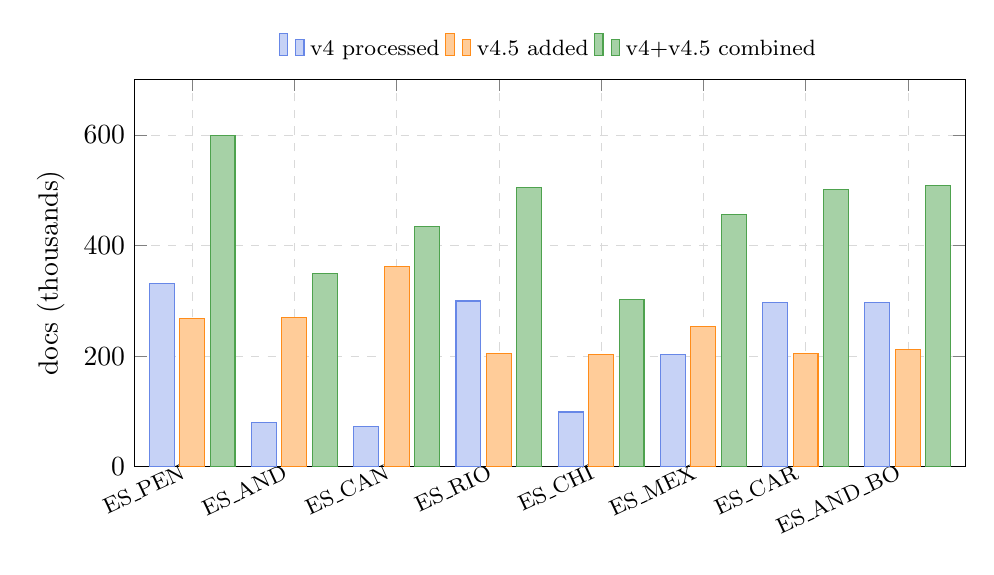
\begin{tikzpicture}
\begin{axis}[
  width=\linewidth, height=6.5cm,
  ybar, bar width=9pt,
  enlarge x limits=0.08,
  symbolic x coords={ES\_PEN,ES\_AND,ES\_CAN,ES\_RIO,ES\_CHI,ES\_MEX,ES\_CAR,ES\_AND\_BO},
  xtick=data,
  x tick label style={font=\footnotesize,rotate=25,anchor=east},
  ylabel={docs (thousands)},
  ymin=0, ymax=700,
  legend style={at={(0.5,1.02)},anchor=south,legend columns=3,font=\footnotesize,draw=none},
  grid=both, grid style={very thin, dashed, black!15},
  nodes near coords style={font=\tiny\bfseries},
  tick align=inside,
]
\addplot+[fill=RoyalBlue!30, draw=RoyalBlue!80] coordinates {
  (ES\_PEN,331.6) (ES\_AND,80.1) (ES\_CAN,72.4) (ES\_RIO,299.6)
  (ES\_CHI,99.0) (ES\_MEX,202.7) (ES\_CAR,297.1) (ES\_AND\_BO,296.9)
};
\addplot+[fill=orange!40, draw=orange!90] coordinates {
  (ES\_PEN,267.8) (ES\_AND,269.3) (ES\_CAN,361.8) (ES\_RIO,204.5)
  (ES\_CHI,202.8) (ES\_MEX,253.8) (ES\_CAR,204.0) (ES\_AND\_BO,211.5)
};
\addplot+[fill=ForestGreen!40, draw=ForestGreen!80] coordinates {
  (ES\_PEN,599.4) (ES\_AND,349.4) (ES\_CAN,434.2) (ES\_RIO,504.2)
  (ES\_CHI,301.8) (ES\_MEX,456.5) (ES\_CAR,501.1) (ES\_AND\_BO,508.4)
};
\legend{v4 processed, v4.5 added, v4+v4.5 combined}
\end{axis}
\end{tikzpicture}
\caption{Per-dialect document counts (in thousands) in the v4 corpus
alone, the v4.5 expansion alone, and the combined v4+v4.5 corpus. The
combined corpus is balanced within a factor of 2 across all eight
varieties.}
\label{fig:balance}
\end{figure}

Before v4.5 the ratio between the largest variety (ES\_PEN, 331k docs)
and the smallest (ES\_CAN, 72k) was 4.6$\times$. After v4.5 the ratio
between ES\_PEN (599k) and ES\_CHI (302k, now the smallest) is
1.99$\times$ --- more than a factor of 2 improvement in balance.

\subsection{Token counts and disk usage}

\begin{table}[h]
\centering
\begin{tabular}{l r r r r}
\toprule
\textbf{Source} & \textbf{Docs} & \textbf{Chars (M)} & \textbf{Tokens (M)} & \textbf{Disk (MB)} \\
\midrule
preseea    & \num{16987}   & 22.2  & 4.43  & 23  \\
coser      & \num{72073}   & 10.3  & 1.93  & 14  \\
lanzarote  & \num{50000}   & 67.5  & 11.52 & 69  \\
cv17       & \num{136349}  & 8.4   & 1.36  & 19  \\
parcan     & \num{100000}  & 65.2  & 11.02 & 333 \\
tweet\_hisp& \num{1600000} & 107.7 & 18.61 & 220 \\
\midrule
\textbf{v4.5 total} & \textbf{\num{1975409}} & \textbf{281.3} & \textbf{48.87} & \textbf{678} \\
\midrule
v4 processed & \num{1679451} & --- & 107.41 & 855 \\
\midrule
\textbf{Combined raw} & \textbf{\num{3654860}} & --- & \textbf{156.28} & \textbf{$\approx$1533} \\
\bottomrule
\end{tabular}
\caption{Document counts, character and whitespace-token counts, and
on-disk sizes of the \texttt{data/raw\_v4/\{source\}} JSONL files for
each v4.5 source. Whitespace tokens are an over-estimate for tweets and
an under-estimate for long transcripts; the $\approx$156M figure should
be interpreted as a rough order of magnitude. Disk usage of the
\emph{HuggingFace cache} for v4.5 is additionally $\approx$\SI{13.4}{\giga\byte}
(the tweet\_hisp parquets), well within the \SI{60}{\giga\byte}
budget.}
\label{tab:tokens}
\end{table}

\subsection{Quality observations}

Inspecting the first record of each source gives a good qualitative
sense of the mix:

\begin{description}[style=nextline,leftmargin=0pt]
  \item[preseea, ES\_CAN] \emph{``¡hola! buenas tardes X muchas gracias
    por por venir bueno vamos a empezar hablando de tu infancia eeh
    cuántos hermanos eran si fuiste feliz si desgraciado etcétera etcétera
    vale pues yo soy de una familia humilde somos cuatro hermanos yo soy
    el menor de todos eeh mi padre se dedicaba a los negocios\ldots''}
  \item[coser, ES\_CAN] \emph{``I2: Antoces=Antonces por eso\ldots''}
    (COSER preserves the rural phonetic rendering \emph{antoces} along
    with the intended form \emph{antonces}.)
  \item[lanzarote, ES\_CAN] \emph{``pues es una reunión que ya estaba
    prevista. no tiene nada que ver con lo ocurrido ayer. enormemente
    interesante para que quienes tenemos responsabilidades\ldots''}
  \item[cv17, ES\_CAN] \emph{``Es una estación que cuenta con cuatro vías
    y dos andenes.''}
  \item[parcan, ES\_CAN] \emph{``DIARIO DE SESIONES PARLAMENTO DE CANARIAS
    I LEGISLATURA\ldots ORDEN DEL DÍA: Constitución del Parlamento de
    Canarias, Investidura del Presidente del Gobierno Autónomo\ldots''}
    (The earliest sessions from 1983 contain OCR-age
    artefacts.)
  \item[tweet\_hisp, ES\_CAN] \emph{``Buenas noches familia!!!''} (with a
    trailing \#hashtag chain from the original tweet).
\end{description}

This spread across formal/institutional (parcan, lanzarote), academic
(preseea, coser), controlled crowdsourced (cv17) and fully colloquial
(tweet\_hisp) registers is exactly the register diversity we wanted per
design goal \textbf{G2}. The downstream classifier will see dialectal
features at every level of formality.

% ==================================================================
\section{Reproducibility}
% ==================================================================

All six downloaders can be re-run independently with:

\begin{lstlisting}[style=shellcode]
# Single-source command
python3 scripts/download_v45_source.py --source <SRC> \
        --max-per-dialect <N>

# Where <SRC> is one of:
#   tweet_hisp preseea coser lanzarote cv17 parcan
\end{lstlisting}

Caches live in \texttt{data/raw\_v4/\{source\}/} and are resumable: a
re-run with a non-empty cache directory returns immediately. To force a
fresh download, delete the \texttt{data/raw\_v4/\{source\}/} directory
first. The HuggingFace cache (used by \texttt{snapshot\_download} for
\texttt{tweet\_hisp}) is at
\texttt{\textasciitilde/.cache/huggingface/hub/datasets--*}.

The six downloaders are deliberately independent so they can be launched
in parallel. On a machine with 8 cores and a 100 Mbps downlink, all six
finish in about 20 minutes (with tweet\_hisp dominating at
$\sim$15 minutes because of its \SI{14}{\giga\byte} parquet download).

Required credentials: an HF access token in the environment variable
\texttt{HF\_TOKEN}, loaded from \texttt{.env} by
\texttt{scripts/download\_v45\_source.py}. Three of the six sources
(PRESEEA, COSER-2024, CV17) are gated and require an accepted dataset
agreement on HuggingFace before the token will authorise the download.

% ==================================================================
\section{Conclusions and next steps}
% ==================================================================

\subsection{What worked}

\begin{enumerate}
  \item \textbf{Six independent downloaders, one per source.} The
        modular design meant that a failure in one source could be fixed
        and re-launched without touching the others, and that the six
        sources could run in parallel across six Python processes.
  \item \textbf{Shared cache + resumability.} Every source's
        \texttt{\_load\_cache} / \texttt{\_save\_cache} pair makes the
        pipeline idempotent. This is critical for sources with long
        downloads like tweet\_hisp: the parquet shards survived a crash
        of the iteration phase.
  \item \textbf{Bypassing \texttt{datasets.load\_dataset} for gated /
        audio-bearing repos.} Two of three failures were solved by
        going directly to the underlying files via
        \texttt{huggingface\_hub.hf\_hub\_download}. This sidesteps both
        the \texttt{torchcodec} dependency and the deprecated-loader-script
        restrictions.
  \item \textbf{Country-grouped parquet skipping for tweet\_hisp.}
        Exploiting the single-country-per-shard property cut the
        iteration time from $>$10 minutes (while still not finishing) to
        $\sim$15 seconds (after the parquets are cached).
  \item \textbf{Explicit dialect metadata over heuristic
        reclassification.} Every document in v4.5 carries a
        \texttt{source} field with a full provenance chain
        (e.g.\ \texttt{tweet\_hisp:spain:santa cruz de tenerife},
        \texttt{coser:fuerteventura}, \texttt{parcan:leg04:ds087}), so
        the dialect label can always be traced back to its evidence.
\end{enumerate}

\subsection{Known limitations}

\begin{enumerate}
  \item \textbf{City diversity in tweet\_hisp.} Because we stop filling a
        dialect as soon as its cap is reached, the 200\,000 ES\_CAN
        tweets in \texttt{tweet\_hisp} all come from a single city
        (\emph{Santa Cruz de Tenerife}), and the 200\,000 ES\_AND tweets
        all from \emph{Almería}. This is fine for coarse dialect
        discrimination but could be improved by round-robin sampling
        across cities.
  \item \textbf{CV17 sentence repetition.} Common Voice prompts are
        repeated many times across speakers; our in-source dedup
        (120-char prefix) reduces but does not eliminate this.
  \item \textbf{parcan OCR noise.} Legislature I (1983--87) sessions
        have visible OCR artefacts
        (\emph{``Afto 'I''}, \emph{``Nº 1''} rendered as \emph{``N2 1''}),
        which the cleaner does not yet fix.
  \item \textbf{Pre-dedup.} The $3.65$M combined count in
        Table~\ref{tab:combined} is a pre-dedup upper bound. The next
        pipeline step (merge + cross-source dedup + length filter) is
        expected to drop this by 10--20\%.
\end{enumerate}

\subsection{Next steps}

\begin{enumerate}
  \item \textbf{Merge + dedup.} Concatenate \texttt{data/raw\_v4/*/} into
        a single \texttt{data/processed\_v45/\{dialect\}.jsonl} per
        dialect, with a 5-gram MinHash dedup step against the existing
        v4 processed corpus, and character-length filtering (drop
        $<\!30$ and $>\!4000$ char outliers).
  \item \textbf{Classifier retraining.} Retrain the BETO+LoRA dialect
        classifier on the merged corpus and measure whether the ES\_CAN
        and ES\_AND F1 scores lift accordingly. The v4 classifier had
        F1 $\approx 0.41$ on ES\_CAN; target for v4.5 is F1 $\geq 0.65$.
  \item \textbf{Validation against the 7 dialectological ranking
        constraints.} Re-compute the pairwise dialect-distance matrix
        with the new corpus and check that the geographically-motivated
        constraints (e.g.\ $d(\mathrm{CAN},\mathrm{CAR}) <
        d(\mathrm{CAN},\mathrm{CHI})$, $d(\mathrm{AND},\mathrm{AND\_BO})
        < d(\mathrm{AND},\mathrm{RIO})$) are satisfied.
  \item \textbf{TDA + eigen-field recomputation.} Re-run the eigenfield,
        Riemannian, and TDA experiments from the v2 algebraic compiler
        on top of the enlarged corpus, and compare the recovered
        spectral signature of ES\_CAN against the one from the noisy v4
        reclassification.
\end{enumerate}

% ==================================================================
\appendix
\section{Code reference}
% ==================================================================

The v4.5 pipeline consists of three files:

\begin{center}
\begin{tabular}{l r l}
\toprule
\textbf{File} & \textbf{LOC} & \textbf{Role} \\
\midrule
\texttt{src/eigen3/downloader\_v45.py} & 1057 & Six downloader functions + registry \\
\texttt{src/eigen3/constants.py}        &  808 & Dialect maps, city sets, confidence scores \\
\texttt{scripts/download\_v45\_source.py} &  83 & CLI dispatcher \\
\midrule
\textbf{Total} & \textbf{1948} & \\
\bottomrule
\end{tabular}
\end{center}

\subsection{Constants updated by v4.5}

The v4.5 expansion added or modified the following top-level names in
\texttt{constants.py}:

\begin{lstlisting}[style=pycode]
# HF dataset IDs
HF_TWEET_HISP_DATASET  = "johnatanebonilla/tweet_hisp"
HF_PRESEEA_DATASET     = "marianbasti/preseea"
HF_COSER_DATASET       = "cladsu/COSER-2024"
HF_LANZAROTE_DATASET   = "StephannyPulido/corpus_registro_canarias"
HF_CV17_ES_DATASET     = "projecte-aina/cv17_es_other_automatically_verified"

# PDF source
PARCAN_BASE_URL             = "https://www.parcan.es/files/pub/diarios"
PARCAN_MAX_LEGISLATURE      = 11
PARCAN_MAX_SESSIONS_PER_LEG = 200

# Mappings
SPAIN_PROVINCE_TO_DIALECT   # 52 provinces + 7 islands + 4 Balearics
CANARIAN_CITIES             # 39 cities/islands
ANDALUSIAN_CITIES           # 53 cities
TWEET_HISP_COUNTRY_TO_DIALECT  # 20 countries
PRESEEA_CITY_TO_DIALECT     # 60 city codes + full names
CV_ACCENT_SUBSTRING_TO_DIALECT # 50 substring rules, ordered

# Per-source confidence weights
SOURCE_CONFIDENCE.update({
    "preseea": 0.95, "coser": 0.95, "tweet_hisp_city": 0.90,
    "lanzarote_cabildo": 0.88, "cv17_accent": 0.85, "parcan": 0.92,
})
\end{lstlisting}

\subsection{Source registry}

All six downloaders are exposed via a single dispatch table:

\begin{lstlisting}[style=pycode]
V45_SOURCES: dict[str, Callable] = {
    "tweet_hisp": download_tweet_hisp,
    "preseea":    download_preseea,
    "coser":      download_coser,
    "lanzarote":  download_lanzarote,
    "cv17":       download_cv17,
    "parcan":     download_parcan,
}

def download_single_source(source, cache_dir, hf_token, max_per_dialect):
    func = V45_SOURCES[source]
    return func(cache_dir, hf_token, max_per_dialect)
\end{lstlisting}

\subsection{Run command summary}

\begin{lstlisting}[style=shellcode]
# All six v4.5 sources, in parallel (run each in its own shell)
python3 scripts/download_v45_source.py --source tweet_hisp --max-per-dialect 200000 &
python3 scripts/download_v45_source.py --source preseea    --max-per-dialect  50000 &
python3 scripts/download_v45_source.py --source coser      --max-per-dialect  50000 &
python3 scripts/download_v45_source.py --source lanzarote  --max-per-dialect  50000 &
python3 scripts/download_v45_source.py --source cv17       --max-per-dialect  50000 &
python3 scripts/download_v45_source.py --source parcan     --max-per-dialect 100000 &
wait
\end{lstlisting}

\end{document}
